\documentclass[]{article}
\usepackage{amsmath}
\usepackage{amssymb}
\usepackage{hyperref}
\usepackage{palatino}
\usepackage{graphicx}
\usepackage{setspace}
\usepackage{amsthm, thmtools}

%Propositions, facts, remarks
\declaretheorem{Fact}
\declaretheorem{Proposition}
\declaretheorem{Remark}


\usepackage[font=scriptsize,labelfont=bf]{caption}
\bibliographystyle{chicago}
\onehalfspacing
\hypersetup{
	colorlinks=true,
	linkcolor=blue,
	filecolor=blue,      
	urlcolor=blue,
	citecolor=blue,
}
\usepackage{comment}

\usepackage{natbib}
\bibliographystyle{chicago}


%opening
\title{Lot Sizes, Welfare and Urban Structure: A View from the United States \\
	Very Preliminary Draft}
\author{James Macek}

\begin{document}
\maketitle	
		
\begin{abstract}
	\scriptsize
This paper considers the welfare effect of minimum lot size regulation, as well as its effect on income segregation. I show that minimal lots are more expensive in productive cities, and this can explain some sorting on income into these cities. I also show that there is negative income sorting on density within these cities, and that sorting is stronger in expensive ones after controlling for other income correlates. Variation in the prices of minimal lots explain both these observations. Motivated by this evidence, I construct a general equilibrium model in which households of heterogeneous incomes choose cities and neighborhoods, value affluent neighbors, and are burdened differently by regulation. A counterfactual deregulation exercise shows significant and progressive gains for renters. The exercise also reveals a surprising result: any productivity gains that occur from the expansion of productive cities are completely nullified by the out-migration of affluent households who prefer regulated neighborhoods. Instead, within city migration matters for renter welfare.
\end{abstract}	
	
	\newpage	
	\section{Introduction}
		
	\paragraph*{}
	
	In recent decades, a large effort has been made to link pervasive US housing regulation with unaffordability. However, these regulations have implications that extend beyond the issue of high housing prices; they presumably slow aggregate growth by limiting density in big cities \citep{hseihmoretti,durantonpugaurbgrowth}. A particular type of regulation -- the minimum lot size -- also causes differences in opportunity and affluence across cities and neighborhoods by excluding those who cannot afford large lots \citep{Song, kulka}. In this paper, I ask how these minimum lot sizes shape aggregate welfare and inequality, as well as their effect on income sorting within and across cities. Understanding minimum lot size restrictions in the macroeconomic context is important because they are ubiquitous across the United States \citep{gyourko2021}. 
	
	\paragraph*{}
	Previous work in the macroeconomics of housing regulation ignores the importance of the income sorting that these regulations cause. The standard story, one echoed by \cite{hseihmoretti} and \cite{durantonpugaurbgrowth}, is that regulations slow aggregate growth by preventing workers from accessing productive cities that are responsible for that growth. However, loosening regulation in expensive cities in the presence of sorting causes high income, productive households to leave, attenuating these negative effects. To motivate this view, I show empirically that the prices of minimal lots are more expensive in productive cities; and this can explain some positive sorting on income into these cities. Moreover, this has broader implications when one accounts for the positive reinforcement of these sorting patterns. Relevant mechanisms include endogenous consumption amenities \citep{diamond2016}, as well as the provision of congested public goods in the zoning context \citep{calabresetal, ineffTiebout}. Unfortunately, these demand side effects have also received little attention in computing the aggregate welfare impacts of regulations. 
	 
	
	\paragraph*{} 
	Focusing on income sorting across cities also masks important sorting happening across neighborhoods \textit{within} these cities. I show empirically that there is negative income sorting on residential density within cities, and that this sorting is significantly stronger in expensive cities after controlling for other income correlates. Variation in the prices of minimal lots explain these observations. This suggests a mechanism driving income sorting that differs from access to public transportation \citep{ccpoortransport}, topographical and historical amenities \citep{parispoor} or filtering dynamics \citep{Gentrificationcycles}. Accounting for within-city geography is crucial for gauging the aggregate welfare impacts of these regulations. Low income households can move toward lightly regulated, high density neighborhoods to avoid large lots, and this movement has spillover effects on housing prices and imposes externalities on neighbors who may value affluent communities. 
	
	\paragraph*{}
	Inspired by this theory and evidence, I construct a general equilibrium model encompassing the metropolitan United States. In the model, households differ on income and choose cities and neighborhoods subject to a varying intensity of regulation. Minimum lot sizes impose a floor on housing consumption required to live in a neighborhood, as in \cite{kulka} or \cite{calabresetal}. Tight regulation excludes the poor by constraining their consumption decisions, whereby increasing neighborhood affluence. The model also incorporates rich heterogeneity across locations along two dimensions. First, cities differ on labour productivity, so that any changes in labour supply across cities affects aggregate productivity. Second, neighborhoods differ both exogenously and endogenously on amenity values; in  particular, these amenity values respond to neighborhood affluence as in \citet{parispoor} or \citet{ghh2013}. This relationship rationalizes the positive correlation between neighborhood amenities and regulation inferred from the calibrated model.

	\paragraph*{}
	I use the model to study the implications of a nationwide elimination of lot size restrictions. The policy change delivers an average gain of $x \%$ for renters and is strongly progressive, while the average landlord loses $z \%$\footnote{These are placeholders for when I implement the model on CoreLogic data. Qualitative descriptions of the results are derived from my prototyped model on Zillow data.}. Allowing amenities to  respond endogenously to the income composition of a neighborhood is responsible for both higher aggregate gains and the progressivity of those gains for renters. The counterfactual also reveals virtually no welfare gains associated with the expansion of productive cities; this is at odds with the macroeconomic literature. Instead, all renters benefit from both the opportunity to consume smaller homes and spillover effects arising from migration \textit{within} cities. The patterns of within-city migration in expensive cities after deregulation look like recent gentrification in the US; affluent households move away from previously regulated neighborhoods and toward dense ones. This \textit{attenuates} the pattern of stronger negative income sorting on density observed in the data. Moreover, low income households move away from high density neighborhoods, decreasing housing prices there. Households who choose to remain in these high density neighborhoods benefit from both
	 spillover effects. 
	
	\paragraph*{}
	I also use this model to evaluate the aggregate welfare implications of uneven reform across space (TBD, placeholder for future work). 
	
	\paragraph*{}
	Using this model to study regulation is challenging because of two methodological issues. First, minimum lot sizes are difficult to measure, especially with broad geographic coverage, because they vary by local jurisdiction and are in most cases not publicly available. I extend the procedure to detect minimum lot sizes used in \cite{Song}, leveraging data on property assessments. These minimum lot sizes enter directly into the calibration of the model, along with housing supply elasticities from \cite{BSH}. Second, inferring the causal effect of neighborhood affluence on amenities is difficult because unobserved amenities likely cause income sorting. I address this endogeneity issue by proposing an instrument based around terrain slopes. It has long been known that neighborhoods with steeper slopes have higher income residents \citep{saiz2010}, but these slopes are likely natural amenities and thus cannot be used as instruments alone. Instead, I assume the amenity value of sloped terrain decays rapidly when moving away from a neighborhood. This justifies the use of a neighborhood-level "donut" design; the income of a neighborhood is instrumented with the slopes of other neighborhoods that are within some distance band. Donut identification designs are prevalent in the IO literature \citep{BFMJPE}, and have been used for different applications in the housing regulation context \citep{anagoletal2021, kulka}.

	\paragraph*{}
	This paper builds upon several strands of literature within  macroeconomics, housing regulation, urban, and public economics. First, this paper challenges the idea that housing deregulation must lead to the growth of productive cities. This is recognized by virtually all work in the macroeconomics of housing regulation as the primary benefit of deregulation \citep{hseihmoretti, durantonpugaurbgrowth, parkho, hop, bunten}. My model yields an opposing conclusion because of household heterogeneity. Stringent regulation in expensive cities affect both the intensive and extensive margin of household labour supply in opposing directions. 
	
	\paragraph*{}
	On the other hand, this paper complements theory and evidence of the effects of housing regulation on housing prices and the structure of cities \citep{MolloyRSUE, gyourkomolloy, turner2014, glaesergyourko2018, bruecknersingh, anagoletal2021, bbheight, mills2005, HILBER2013, op2014}, and particularly the minimum lot size \citep{zabel, Song, kulka, KSC, griesonwhite, WHITE1975}. Using both a discontinuity design and a model, \cite{Song} and \cite{kulka} show extreme income and racial sorting on minimum lot sizes, and \cite{KSC} show that height restrictions and unit density restrictions work in tandem to increase housing prices. I differ from this work along several dimensions; these papers do not incorporate endogenous amenities\footnote{\cite{Song} directly models preferences over minimum lot sizes in a discrete choice model. This may be thought of as a stand-in for endogenous amenities. However, minimum lot sizes are likely correlated with unobserved demand factors, and no instrument is used in the structural model to address identification of demand parameters. Moreover, directly modeling preferences over minimum lot sizes results in a model with no fiscal externalities, and this misses a key channel that affects welfare \citep{hamilton1976, calabresetal}. On the other hand, \cite{KSC} use a discontinuity design to identify neighborhood demand for a low density of housing units. I posit an alternative specification -- demand for high income neighbors.}, they do not model heterogeneous city technologies, and they limit the spatial scale of their counterfactuals; that is, they do include spillover effects of deregulation on neighborhoods with little or no lot size regulation, such as in the downtowns of expensive cities. The main message of this paper is that each matter for welfare consequences. 
	
	\paragraph*{}
	This paper also builds upon relatively recent work studying urban sorting on income and other demographics \citep{diamond2016, bshartley2020, couturehandbury, Coutureetal, superstarcities, su2021, citysizewagegap, Gentrificationcycles, FogliGuerrieri, ccpoortransport, parispoor}. I add to this literature by providing theory and evidence that regulation causes income sorting on density in cities with high housing prices. In addition, a major lesson from this literature is that exogenous demographic changes can be positively reinforced by the endogenous supply of amenities. I also highlight the role of endogenous amenities in both sorting patterns and welfare gains after deregulation, and think carefully about identifying this relationship.
	
	\paragraph*{}
	Lastly, this paper provides an update to the exclusionary zoning literature \citep{hamilton1976, calabresetal, keepingpeopleout, ineffTiebout, barcoate}. In my model, the relationship between amenities and neighborhood income composition can be similarly interpreted in the context of local public goods. However, I do not endogenize the choice of regulation, and instead consider it as a lever than can be freely changed by some central government. One benefit is that regulation in my model is calibrated to match the data, rather than set to be an outcome of a voting model that may be mispecified.
	
	\paragraph*{}
	This draft is organized as follows. Section \ref{Section:Evidence} introduces the evidence, and Section \ref{Section:Model} introduces the final model I will use with CoreLogic data, when available. I also show that the empirical facts arise endogenously from the simple model. 


	\section{Data and Motivating Evidence}\label{Section:Evidence}

	\paragraph*{}
	In this section, I argue that variation in the stringency of minimum lot size regulation both within and across cities can explain broad patterns of income sorting we see in the data. The importance of this observation extends far beyond positive economics -- it informs how these patterns might change in response to deregulation, which neighborhoods benefit from these changes, and how these benefits comprise the aggregate welfare consequences of the policy. I discuss this in more detail after introducing the facts. 
	
	\paragraph*{}
	 To establish these facts, I draw on numerous sources of data. I take household income and other demographics from the pooled 2016-2020 ACS, census housing counts from the 2020 census, and various amenity data from the National Neighborhood Data Archive (NaNDA). I combine this with data on recent assessments and housing transactions\footnote{For this draft, I use the Zillow 2015 assessments in anticipation for CoreLogic. Note: these updated facts are for the 2020 version of the census and 2016-2020 version of the ACS, to be used with CoreLogic. I also use measured minimum lot sizes from Zillow. This will be replaced with CoreLogic data when ready. There should not be many differences between the data. }. This is the main source used to estimate both minimum lot sizes and the prices of those minimal lots. The primary unit of analysis is the 2020-definition census block group; in what follows, this is the definition of a \textit{neighborhood}. Each neighborhood is matched to a unique 2013-definition Metropolitan Statistical Area (MSA) on centroids; these are referred to as \textit{cities}. There are approximately 196,000 neighborhoods allocated to 377 cities in the main estimation sample.   
	
	\paragraph*{}
	I establish two broad facts. The first links residential density (the number of housing units per unit of land) to income within cities, hearkening back to literature that seeks to explain why US downtowns are poor \citep{Gentrificationcycles, ccpoortransport, parispoor}. Since residential density is directly affected by lot sizes, the second fact links both observations to variation in the stringency of lot size regulation, both within and across cities. Taken together, these suggest that regulation has fundamentally altered urban structure. I start with Fact \ref{FIncomeDens}. 

\begin{Fact}\label{FIncomeDens}
	(The geography of residential income sorting)
	\begin{enumerate}
		\item Within cities, there is a negative relationship between household income and residential density. 
		
		\item Cities with high housing prices exhibit a stronger income-density gradient after controlling for income correlates, such as building age, access to public transportation, and various observed amenities.
	\end{enumerate}
\end{Fact}

\paragraph*{}
To show the first part of Fact \ref{FIncomeDens}, I order neighborhoods in each city by the density of housing units (dividing the 2020 census household count with the measured land mass of the neighborhood). Since block groups are drawn to have roughly similar populations, larger cities have more neighborhoods in the sample. I normalize this ranking so that it forms an even partition of the unit interval within each city, ensuring cities of differing sizes are comparable. A linear regression of log average household income against this ranking (with city fixed effects) reveals a striking negative relationship -- moving from the least to the most dense neighborhood in an average city cuts income roughly in half. 

\paragraph*{}
Residential density is an endogenous object -- it reflects several underlying factors that must be driving income sorting. High density neighborhoods may contain buildings that are old and dilapidated, thus attracting the poor \citep{Gentrificationcycles}. These neighborhoods might also be easily accessible by public transportation, which the poor are more likely to use \citep{ccpoortransport}. The second part of Fact \ref{FIncomeDens} says that controlling for these underlying factors reveals a leftover income-density gradient that is \textit{stronger} in larger, more expensive cities. To show this, I split the main estimation sample into one containing cities that are in the top quartile of housing prices, and one associated with the bottom quartile. I consider the following partial linear model over neighborhoods $i$ and cities $c$ in each sample
\begin{equation}\label{Specification:IncomeSortingStrong}
	\log(Income_{ic}) = \mathbf{S}(RankedHousingDensity_{ic}) + \sum_{x \in \mathbf{Controls}}\beta_{x}x_{ic} + \epsilon_{ic}
\end{equation}
where $\mathbf{S}$ is a cubic spline and the $\beta_{x}$ are coefficients to be estimated. $\mathbf{Controls}$ include building age, shares of individuals using cars and public transport, density of public transportation, average commute time, household size, density of bars and coffee shops, among others; I include the full list below. All variables are demeaned by the city average. I estimate two versions of Equation \eqref{Specification:IncomeSortingStrong} on each sample: one with no controls ($\beta_{x} = 0$ for every $x$), and one including the full set. The objective is to document the shape of the function $\mathbf{S}$ across samples, and I do so in Figure \ref{Figure:IncomeSortingStrong}. 

\begin{figure}[!ht]
	\begin{center}
		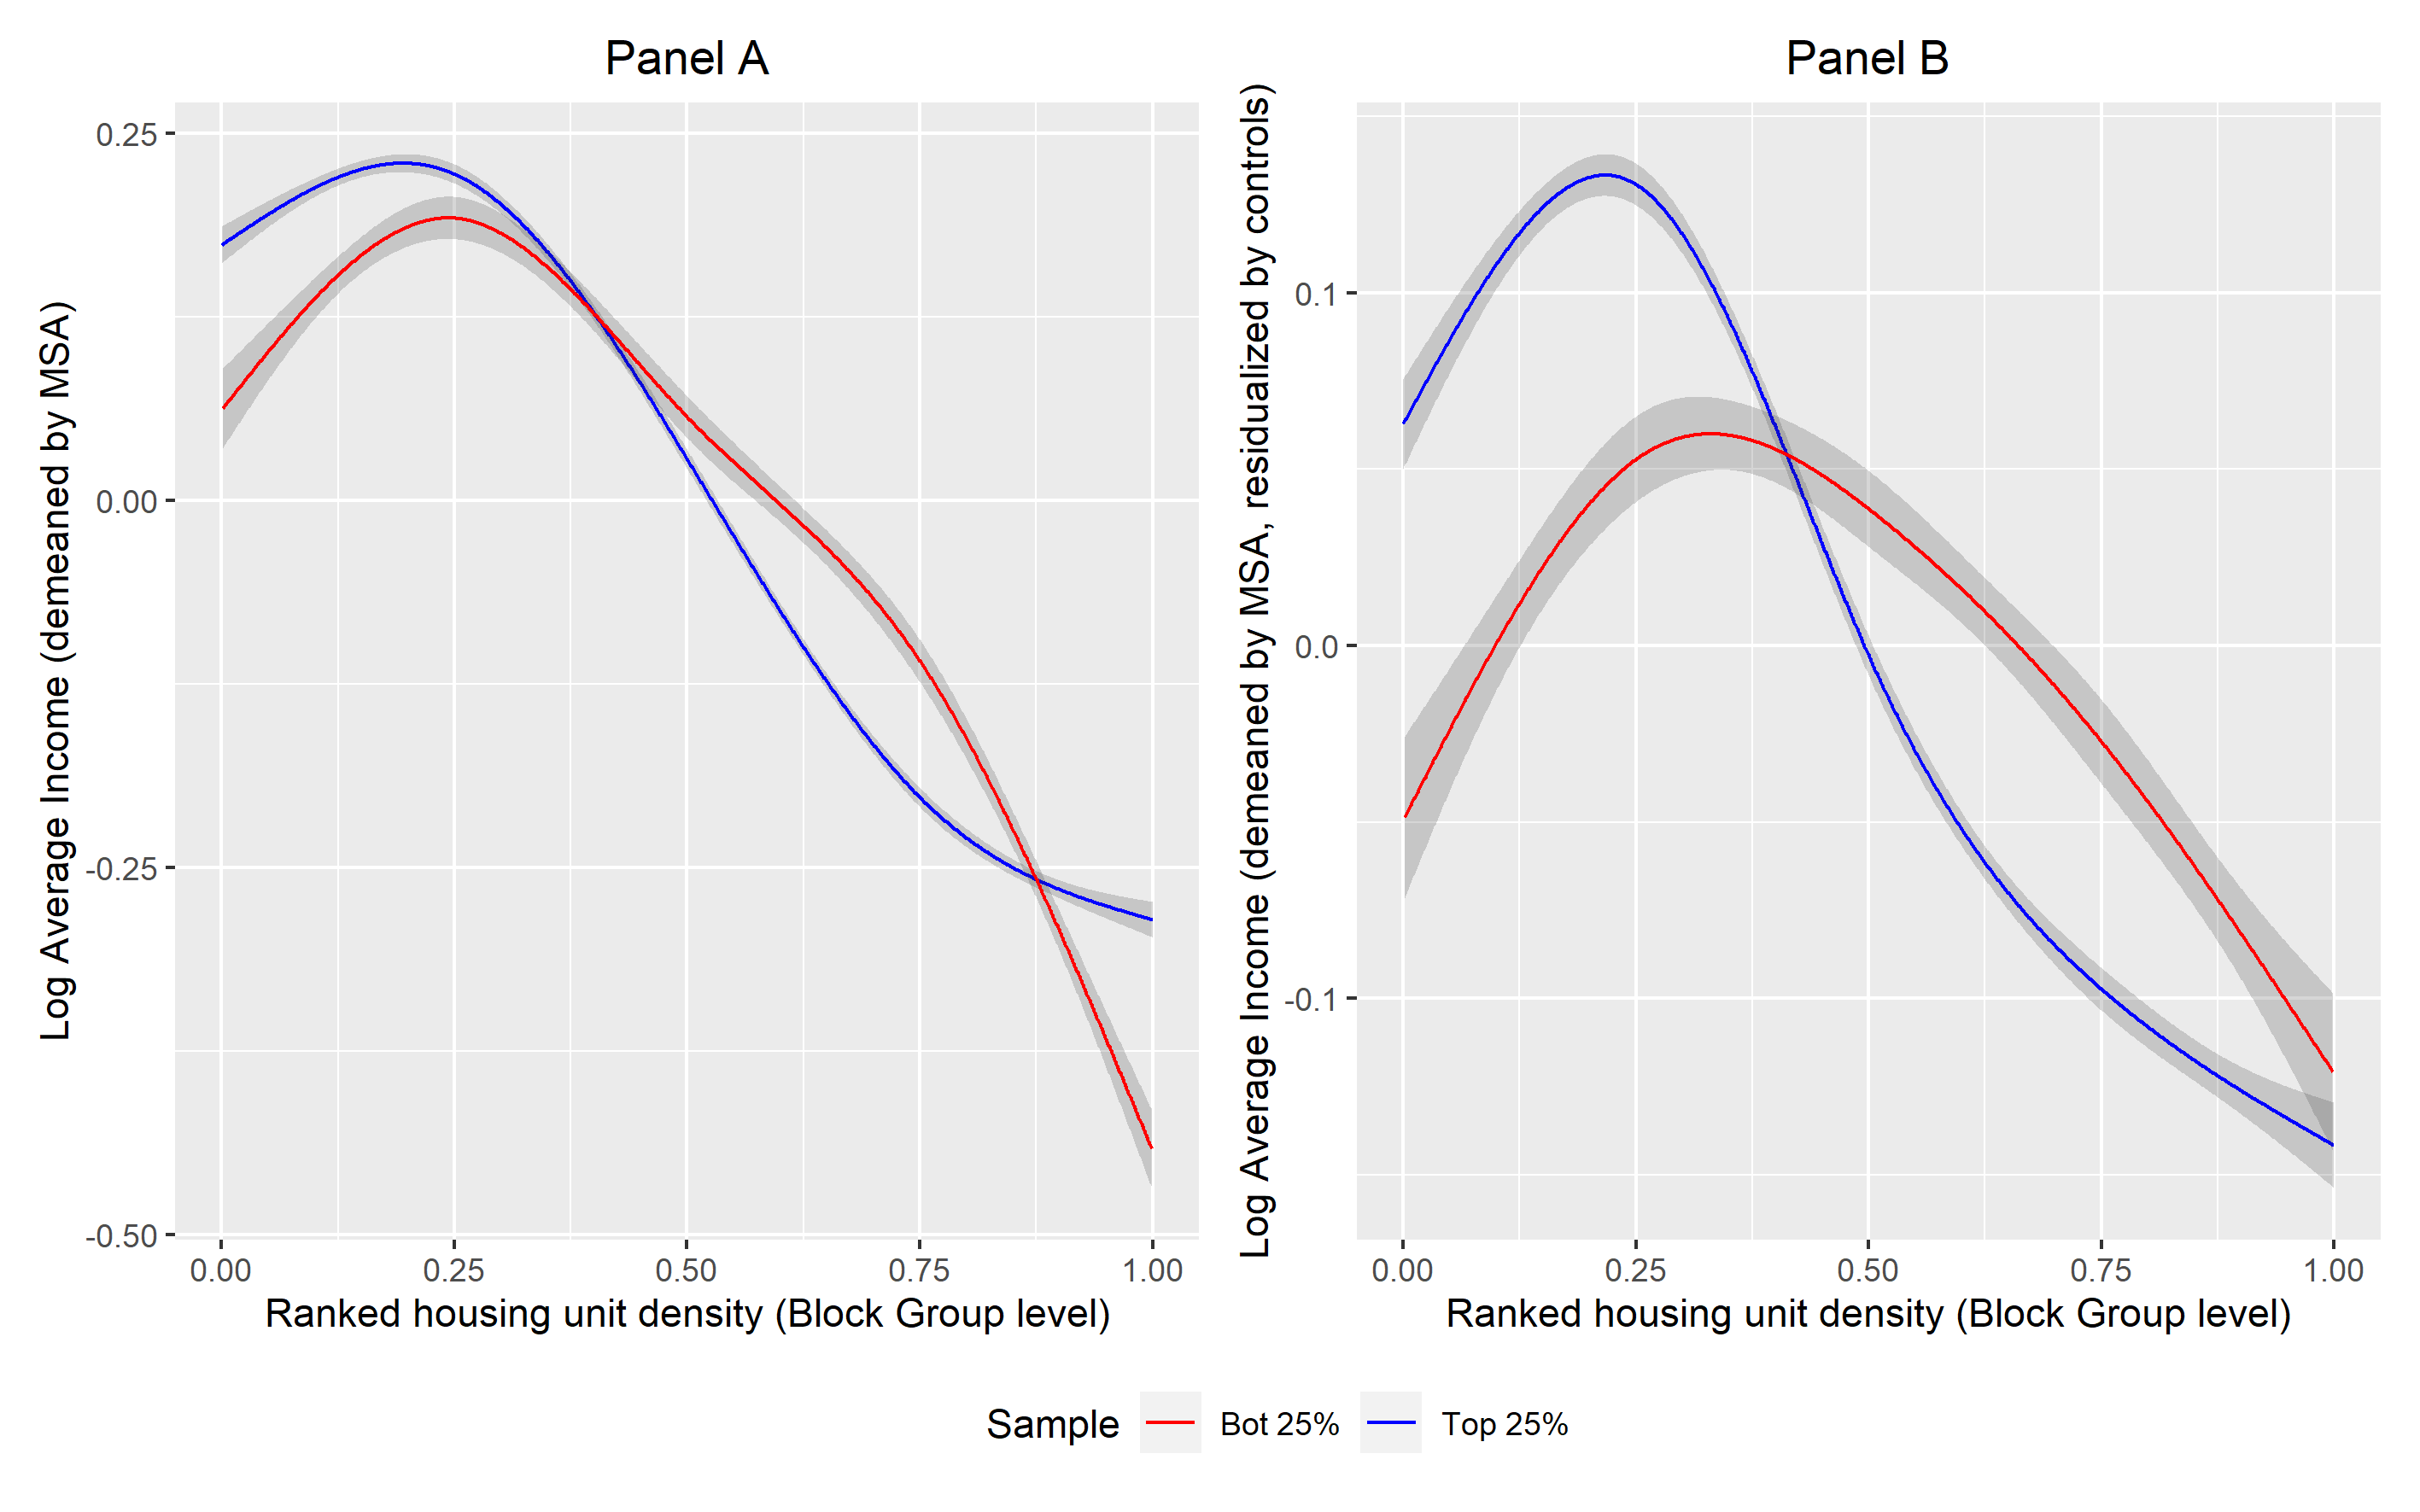
\includegraphics[width=\textwidth]{income_combined.png}
		\caption{Plot of cublic spline $\mathbf{S}$ from Equation \eqref{Specification:IncomeSortingStrong} with 5 knots, estimated with the \textit{mgcv} package in R \citep{gampackage}. 95\% confidence sets are reported. Panel A reports the model with excluded controls, while Panel B includes the model with the full set. The full set of controls are building age, household size, share of households using public transport to commute, share of households using cars to commute, and average travel time from the ACS; density of performing arts, spectator sports, casinos, recreational activities, restaurants, fast food, bars and coffee shop establishments from NaNDA; and the density of EPA toxic releases and the density of public transport stops from NaNDA. All variables from the ACS vary at the block group level, and at the tract level for NaNDA.  }\label{Figure:IncomeSortingStrong}
	\end{center}
\end{figure}

\paragraph*{}
Panel A of Figure \ref{Figure:IncomeSortingStrong} reports $\mathbf{S}$ for expensive cities (in blue) and inexpensive cities (in red) with excluded controls. There is a clear negative relationship across samples. However, there is not much difference in the income-density gradient; if there where, one would expect that high density neighborhoods in expensive cities would be relatively less affluent. Visually, this would correspond to the blue curve being below the red curve for most neighborhoods the top half of the density distribution. Instead, this pattern becomes clearly visible in Panel B after accounting for other observable characteristics of these neighborhoods that cause income sorting. Panel B also shows that the differences in the gradients are large. For example, an observationally equivalent neighborhood in the $75$th percentile of the density distribution would be roughly $7.5$\% poorer relative to the mean in expensive cities, and similarly $7.5$\% richer relative to the mean for neighborhoods in the $25$th percentile. 

\paragraph*{} 
Clearly, there must be some other mechanism that both correlates with density and drives income sorting that was not accounted for. This mechanism must also act differently in the largest, most expensive cities in order to rationalize differences in the income-density gradients. It has long been argued that productive and expensive cities are more likely to impose stringent regulation \citep{HILBER2013,parkho, durantonpugaurbgrowth}. I echo a similar message and make an additional argument: within-city variation in regulation across neighborhoods is fundamentally different in expensive cities. I end with Fact \ref{FStringency}. 

\begin{Fact}\label{FStringency}
	(The geography of minimum lot sizes)
	\begin{enumerate}
		\item  Low density neighborhoods in expensive cities exhibit relatively higher regulatory stringency than cheap cities. Conversely, high density neighborhoods in expensive cities are relatively less stringent. This explains the stronger income-density gradient in expensive cities. 		
		\item  The stringency of lot size regulation is significantly higher in expensive cities. This explains some positive income sorting into these cites. 
	\end{enumerate}
\end{Fact}
	
	\paragraph*{} 
	To show Fact \ref{FStringency}, I first establish a clear definition of regulatory stringency that will be derived in the model of Section \ref{Section:Model}. This definition relies on two simplifying assumptions. Suppose we have measured a minimum lot size $l_{ic}$ (in acres) in some neighborhood $i$, and suppose exactly one household must rent at least the amount of structure on that minimal lot to live in the neighborhood\footnote{In the empirical work, I allow for duplexes, triplexes and quadriplexes by making simple adjustments to the measured minimum lot sizes.}. Implicitly, this means that the minimum lot size is uniform in $i$. In addition, assume that structure is supplied at a rate proportional to the size of the lot within $i$, and that the rental rate for a unit of structure is also uniform within $i$ and roughly proportional to the market value of the house. I define the \textit{stringency of minimum lot size regulation} $I_{ic}$ as the value of structure on a minimal lot  where
	\begin{equation}\label{observedStringency}
		I_{ic} = V_{ic}l_{ic}
	\end{equation}
	where $V_{ic}$ is the housing value per acre in neighborhood $i$ and city $c$, observed from the transactions data\footnote{This transactions data is from Zillow and limited to the 2008-2012 period (which lined up with my previous choice of ACS data), and lot sizes are measured as the most recent assessment data as of 2015. The associated CoreLogic data will be from 2016-2020 to match up with the most recent assessments as of 2022.}. In the model, higher stringency levels imply stronger income sorting -- households with low income are forced to spend a fraction of their income to rent the minimal lot beyond what they would if they could choose their housing consumption freely. 
	
	\paragraph*{}
	The first part of Fact \ref{FStringency} says that the stronger income-density gradient in expensive cities is met with a similarly stronger stringency-density gradient, suggesting that regulation is an underlying causal factor. To show this, I alter the regression in Equation \eqref{Specification:IncomeSortingStrong} such that the dependent variable is instead $I_{ic}$ demeaned by the  average in $c$. The objective is essentially the same as in the exercise in Panel A of Figure \ref{Figure:IncomeSortingStrong}: to plot the function $\mathbf{S}$ associated with this regression for both city samples and compare them. I do so in Panel A of Figure \ref{Figure:StringencyStrong}, with controls excluded. 
	
	\begin{figure}[!ht]
		\begin{center}
			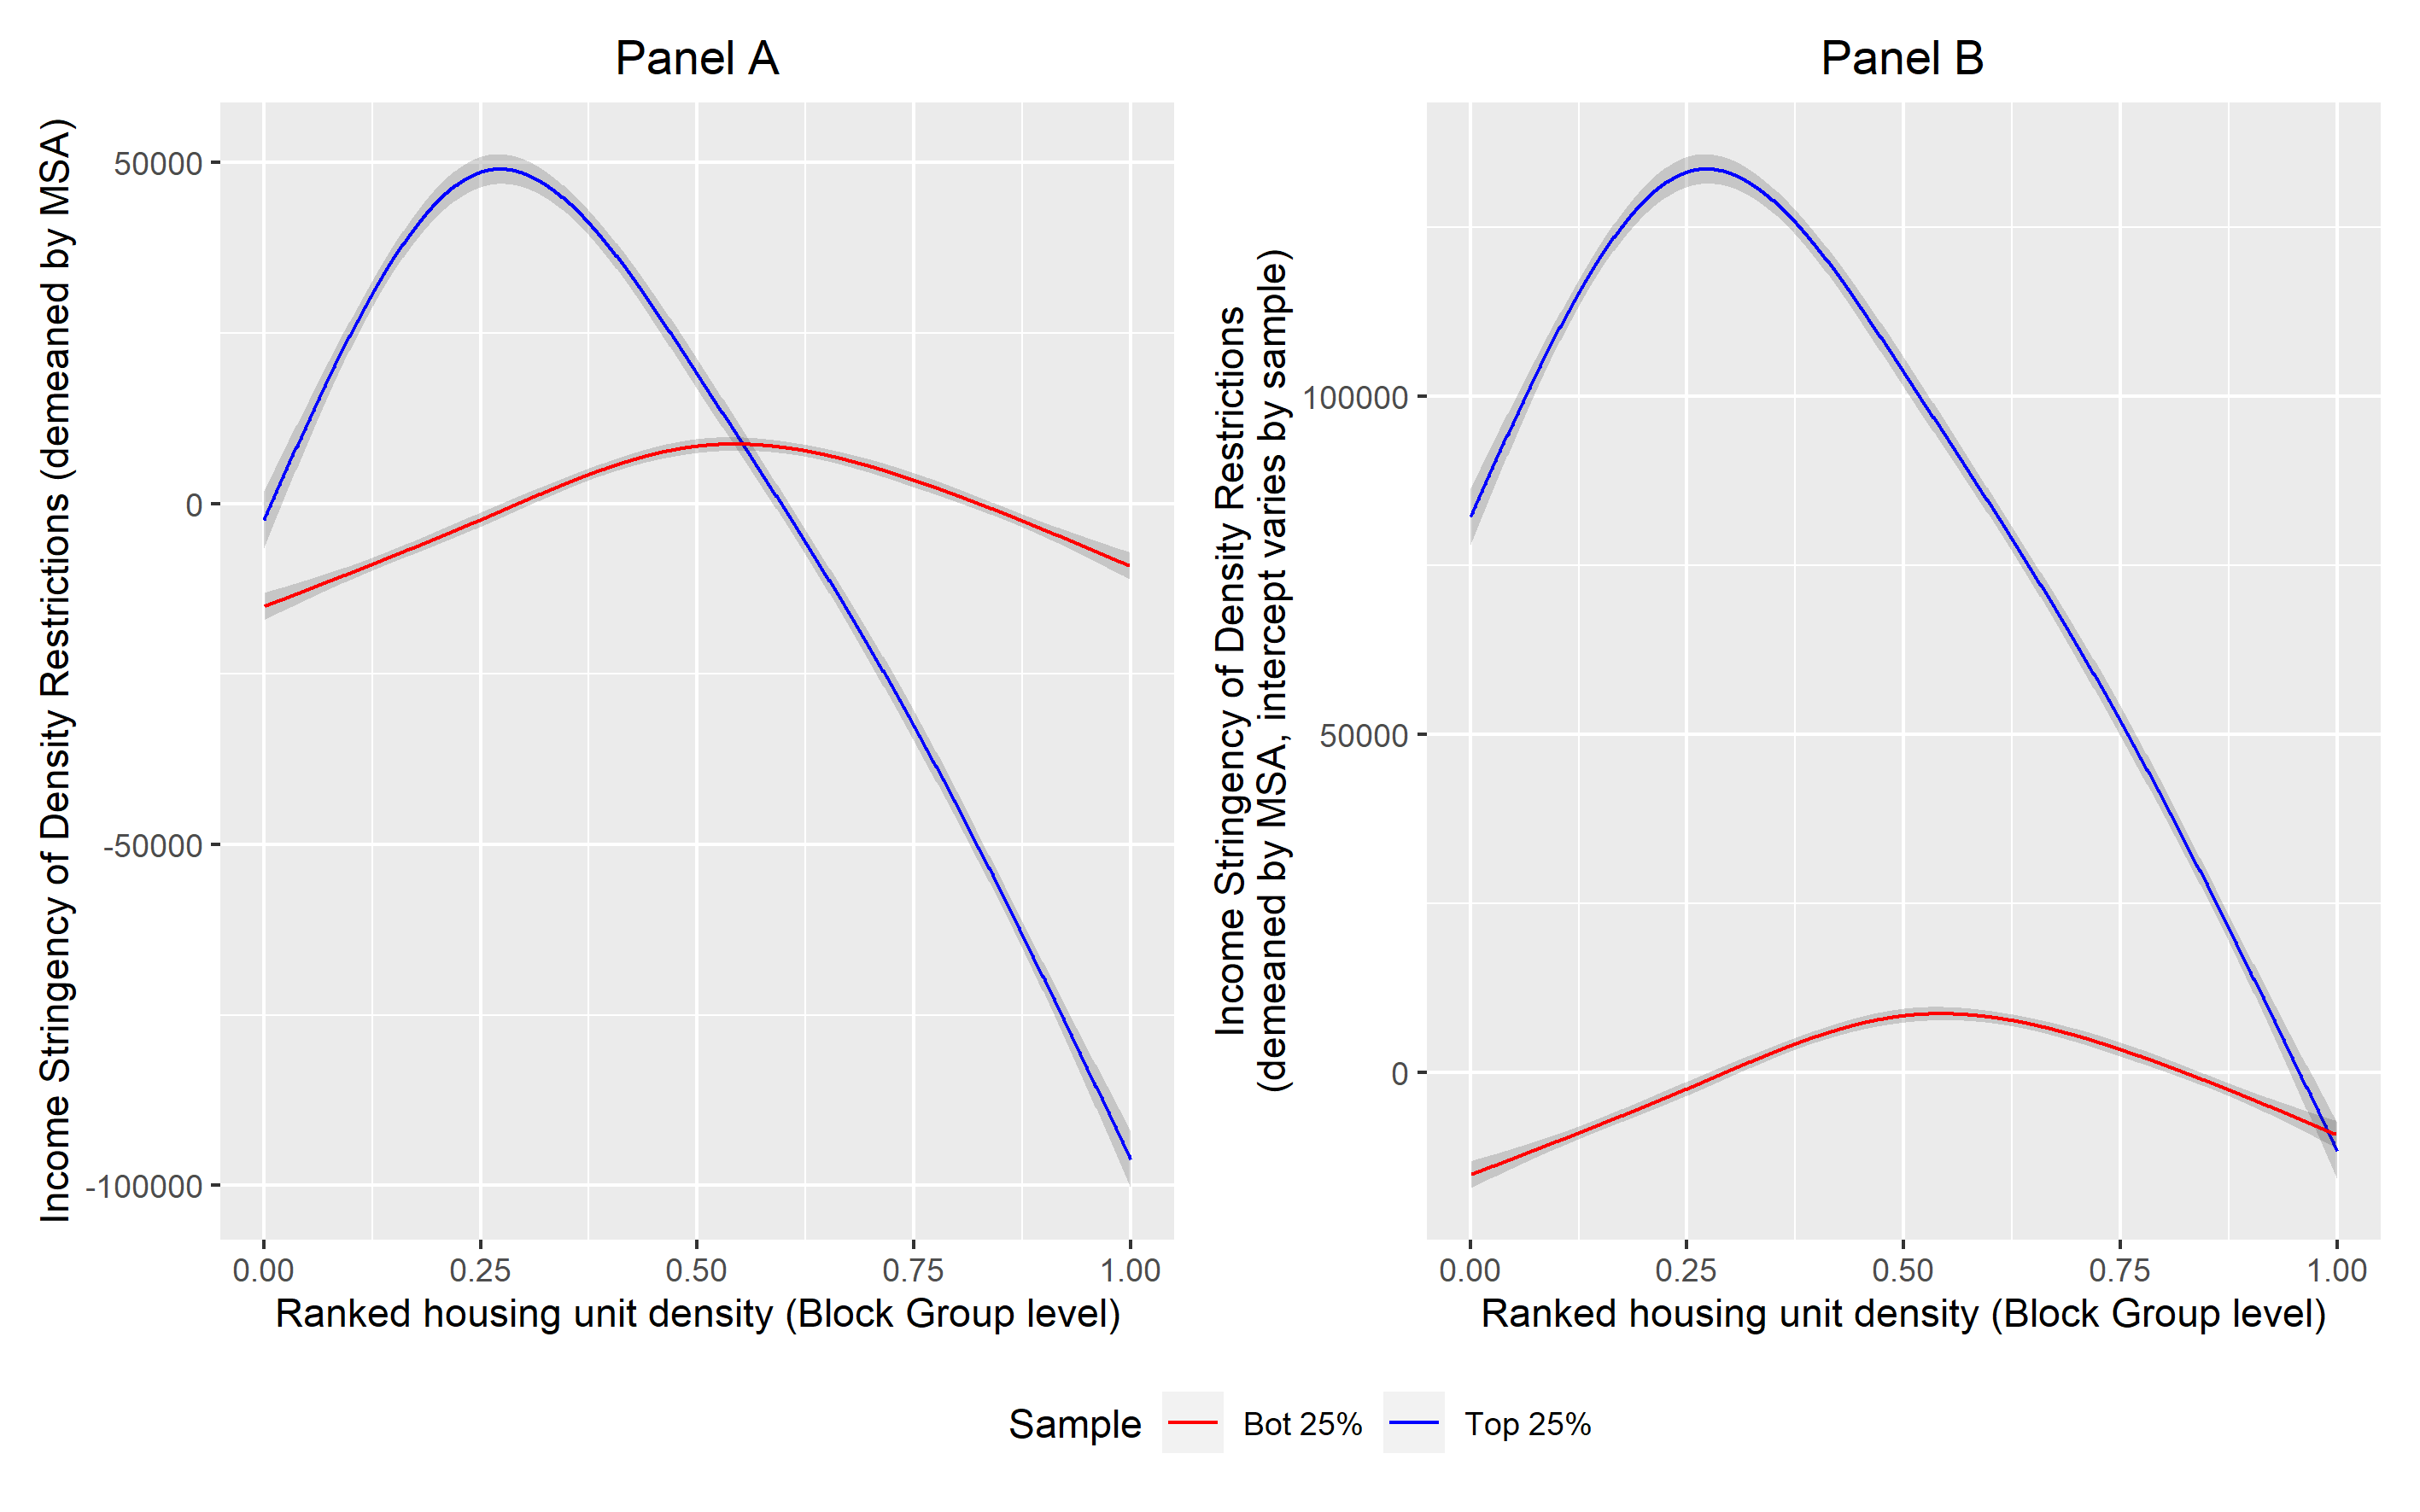
\includegraphics[width=\textwidth]{incomestringency_combined.png}
			\caption{Plot of cublic spline $\mathbf{S}$ with 5 knots, estimated with the \textit{mgcv} package in R \citep{gampackage}. The specification in Panel A replaces log income in Equation \eqref{Specification:IncomeSortingStrong} with regulatory stringency in Equation \eqref{observedStringency} and \textit{excluded} controls, demeaned by city and measured in 2012 US dollars. The residualized version of this regression (mirroring Panel B of Figure \ref{Figure:IncomeSortingStrong}) is omitted as they look qualitatively identical. 95 \% confidence sets are reported. Panel B repeats the same regression while allowing the average stringency to vary by sample. In other words, the blue curve is shifted upward by a constant. }\label{Figure:StringencyStrong} 
		\end{center}
	\end{figure}

	\paragraph*{}
	Panel A of Figure \ref{Figure:StringencyStrong} reveals a strikingly similar pattern to Panel B of Figure \ref{Figure:IncomeSortingStrong}: high density neighborhoods in expensive cities exhibit relatively less stringency, and low density neighborhoods relatively higher stringency. A qualitatively similar pattern holds when conditioning on controls, so the associated plot is omitted. These differences are large. The highest density neighborhood in an expensive city has the value of a minimal lot that is almost $\$ 100,000$ lower relative to the city mean. At the 25th percentile, expensive cities have a value that is roughly $\$ 50,000$ greater. These differences represent a substantial proportion of the average value of a home. Conceptually, the differences in relative stringency at different points along the density distribution accompany differences in the \textit{types} of residential structures that appear. Think about the densest neighborhood in Los Angeles -- most of the housing units are in large structures, where there is no concept of a minimum lot size\footnote{Regulatory authorities could impose minimum floorspace requirements for units in large residential structures. However, these units tend to be consistently smaller than single family homes.}. Contrast this with a cheap city like Memphis, where the densest neighborhoods consist of marginally smaller single family homes. 
	
	\paragraph*{}
	The second part of Fact \ref{Figure:StringencyStrong} says that expensive cities have higher levels of stringency in an average neighborhood. This observation can explain some income sorting into expensive cities to the extent that this reflects sorting on skills or other household attributes \citep{diamond2016, citysizewagegap}. In Panel B of Figure \ref{Figure:StringencyStrong}, I show this by repeating the same regression as in Panel A while allowing the average stringency across neighborhoods to vary across the two samples. The figure shows that, in practically every neighborhood, average stringency levels are higher in expensive cities. A typical neighborhood in the middle of the density distribution has a price of a minimal lot approximately $\$100,000$ greater in expensive cities. This gap in stringency disappears only in the highest density neighborhoods. 
	\paragraph*{}
	It may be unsurprising that expensive cities have more expensive minimal lots. However, the measure $I(i)$ is the product of two forces in Equation \eqref{observedStringency} -- while expensive cities naturally have higher housing prices per acre, they also tend to have smaller minimum lot sizes. The gap between the value per acre and the minimum lot size in productive cities likely reflect political economy forces; these arise endogenously in certain models of housing regulation, such as \cite{parkho} or \cite{HILBER2013}. Interestingly, these models cannot explain the stringency-density gradient within expensive cities, as they would predict neighborhoods with the best commuter accessibility to productive employment centers to have the highest level of regulation. While the objective of this paper is not to justify an alternative explanation, I can speculate. In the neighborhoods to allow for high density structures (like in high density neighborhoods in expensive cities), the power for local homeowners to limit density is low. It may be because these neighborhoods are not fiscally decentralized\footnote{For example, San Francisco has one board responsible for city planning in the entire county. When approving projects, they commonly express interest in the welfare of renters, not just homeowners. The same might not be said for other neighboring jurisdictions like Palo Alto. A related idea is that downtowns are poor because the rich like to escape redistributive policies, as hypothesized in \cite{NechybaWalsh}.}, and this matters for stringency \citep{ineffTiebout}. It may also be because these neighborhoods predate the enforcement of regulation and where "locked in" to high density\footnote{I thank Will Strange for this suggestion.}. Whatever it may be, the purpose of this paper is to show why this variation in regulation matters for policy. I do so below. 
	
	
	\paragraph*{Welfare Consequences of Deregulation} Facts \ref{FIncomeDens} and \ref{FStringency} inform how large scale deregulation might affect the welfare of spatially mobile households. On one hand, the macroeconomic literature emphasizes that housing regulation limits aggregate labour productivity because it limits the size of productive cities \citep{hseihmoretti, durantonpugaurbgrowth}. This assertion is muddied by the fact that labour supply to any given city depends both on the number of households and the labour supply per household. If regulation causes productive cities to have a high labour supply per household as suggested by Fact \ref{FStringency}, then any productivity gains from deregulation could be offset by the out-migration of affluent households. Indeed, eliminating all minimum lot sizes in the forthcoming model finds essentially no gains to aggregate productivity\footnote{From old draft on Zillow data. Subject to change, although it shouldn't.}. In fact, across-city migration does not influence the welfare effects of deregulation at all\footnote{This is measured by comparing the counterfactual under a full model and one where across-city migration is restricted.}.
	
	\paragraph{}
	On the other hand, within-city variation in income and lot size stringency highlighted in Facts \ref{FIncomeDens} and \ref{FStringency} suggest \textit{which} neighborhoods will benefit from deregulation. In expensive cities, movement of affluent households from previously regulated, low density neighborhoods and towards high density ones may have spillover effects on the amenities offered in these high density neighborhoods. At the same time, the outflow of many low income households from high density neighborhoods may decongest housing markets. This is exactly what I find in the deregulation exercise; high density neighborhoods of expensive cities experience large gains in amenity values and lower housing prices relative to low density neighborhoods, despite the former neighborhoods having considerably lower levels of regulation. I also show that this within-city migration explains roughly $20\%$ of the aggregate welfare gains accruing to renters\footnote{The other $80\%$ comes from the option value of being able to consume smaller homes.}. In the following section, I construct the model used to arrive at these welfare calculations.

	\paragraph*{}
Before continuing, I note that there are many arbitrary choices used to construct the data to generate these facts. In Appendix \ref{Appendix:Robustness}, I show that the facts are robust to a host of sample definitions, weighting schemes and other contexts. I also discuss instances where the facts do not hold; for example, when replacing the housing unit density ranking with distance to the central business district. 
	
	\section{Model}\label{Section:Model}
	\paragraph*{}
	In this section, I introduce a simple theoretical framework that will be able to rationalize Facts \ref{FIncomeDens} and \ref{FStringency}, and be used to evaluate the consequences of large scale deregulation. 

\paragraph*{Geography}
I consider a finite set of cities $C$ indexed by $c$, which map to MSAs in the data. These cities are self-contained labour markets; that is, I do not allow households to access productive technologies outside of the city for which they reside. Each city $c$ has an exogenous finite set of neighborhoods $N(c)$. I use the index $i$ to denote a typical neighborhood from any city, $i \in \cup_{c \in C}N(c)$, and define the map $C(i)$ to be the city associated with $i$. Here, neighborhoods are defined to be census block groups. Each of these neighborhoods have an exogenous amount of land $T_{R}(i)$ that is available to developers for the production of housing services. 

\paragraph*{Developers}   
In anticipation of households making choices over neighborhoods to reside, I assume that exactly one household can occupy one housing unit. In a standard model of housing supply, developers are indifferent to producing any number of housing units\footnote{See, for example, the housing supply model in \cite{BSH}.}. This means that the number of housing units can be arbitrarily large; as large as the number of households who choose the neighborhood in equilibrium. Complicating this problem is the minimum lot size $\bar{l}(i)$ and the regulation of how many housing units can occupy each lot. To make the exposition clear, I start with preliminaries. In each neighborhood, I partition residential land $T_{R}(i)$ into equal sized \textit{parcels} of normalized mass $1$. That is, there are a mass $T_{R}(i)$ of parcels. These are the units of land that the representative developer uses to produce structure. These parcels can be \textit{split} into lots, and lots are a fundamental unit by which regulation operates. Each lot can hold a regulated maximum $\bar{h}(i)$ housing units. For example, $i$ may allow duplexes, so that $\bar{h}(i) = 2$. Then, $\bar{l}(i)/\bar{h}(i)$ is the minimum amount of land per housing unit in $i$. Let $l(i)$ denote this minimum land per housing unit, which will be the main object I work with hereafter\footnote{An implicit assumption is that there is no material difference between single family homes on small lots or multifamily homes on large lots. This is obviously untrue if households have lower demand for multifamily units, all else equal. I control for these implicit quality differences using a hedonic regression introduced in Section (xx).}. $l(i)$ may be zero if the neighborhood is unregulated, and is constructed from lot size data using a procedure in Section (xx). 

\paragraph*{}
Given a parcel in $i$, developers choose the total amount of structure $A(i)$ that can occupy it in a standard way. That is, they use a neighborhood-varying Cobb-Douglas technology over land and capital, facing a perfectly elastic supply of that capital at rate $r$. This yields the neighborhood-level housing supply function per unit of land
\begin{equation}\label{supplyfn}
	A(i) = \lambda(i)P(i)^{\epsilon(i)}
\end{equation}
where $P(i)$ is the price of a unit of housing stock, $\epsilon(i)$ is the supply elasticity in block group $i$ and $\lambda(i)$ is a supply shifter net of capital costs. In a world without minimum lot sizes, the developer is indifferent to allocating this structure across housing units; there can be many small houses or few large ones, provided the total stock is given by \eqref{supplyfn}. Instead, if developers respect the minimum lot size, the minimum amount of housing stock per housing unit $A^{\star}(i)$ must be

\begin{equation}\label{minstructure}
	A^{\star}(i) = \lambda(i)P(i)^{\epsilon(i)}l(i)
\end{equation}

\paragraph*{}
I take the quantity $A^{\star}(i)$ as a minimum amount of housing stock required to be purchased to live in neighborhood $i$. The value of this minimum quantity $P(i)A^{\star}(i)$ is the model equivalent to the observed stringency of regulation in Equation \eqref{observedStringency} used to construct Fact \ref{FStringency}. Households with little disposable income after paying for this minimum quantity are forced to purchase more than what they would if this quantity could be freely chosen. This arises naturally from the household's consumption problem.\footnote{Equation \eqref{minstructure} also reveals the material difference between lot size regulation and other regulations studied in contemporary quantitative models. Contrast the equation with the standard Floor Area Ratio restriction in \cite{bruecknersingh}, which puts limits on housing \textit{stock} per parcel. Here, there are no stock density  limits -- just limits on the number of housing units (or households) that can occupy a parcel. This distinction is forcefully argued in \cite{griesonwhite}.}

\paragraph*{Household Consumption}
Households have Cobb-Douglas preferences over a freely traded, homogenous good $g$ (with a normalized price of 1 dollar) and housing $A$. Households differ on \textit{income type} indexed by $z \in Z$, where $Z$ is finite. Alternatively, $z$ is the labour supply of the household. Crucially, the income type is observed by the econometrician. Accompanying these types, I introduce unobserved heterogeneity in \textit{transfers}, indexed by $\tau \in \mathbb{R}_{+}$.  I introduce this heterogeneity because I am confronted with the reality that the types of households that the model predicts would be completely priced out of the housing market appear in certain stringently regulated neighborhoods.  This can be for many reasons, including model mispecification, unobserved wealth (especially housing wealth), housing subsidies, and unobserved permanent income; $\tau$ should be loosely interpreted as an amalgamation of each. Type $z$ households with unobserved transfer $\tau$ have a disposable income $z\tau$ to spend on housing and other consumption.

\paragraph*{}
Let $\bar{L}(z, \tau)$ be the mass of type $(z, \tau)$ households. Deferring neighborhood choice for a moment, suppose a household of type $(z, \tau)$ has chosen $i$.  Given the city $C(i)$, households receive a wage $w(C(i)) := w(i)$ per effective unit. Given this wage, the household of type $(z, \tau)$ chooses consumption $g$ and rents housing $A$ to maximize
\begin{equation}\label{utility}
	\max_{A, g} A^{\beta}g^{1-\beta}
\end{equation} 
subject to $A \geq A^{\star}(i)$ and $P(i)A + g \leq w(i)z\tau$. Let  $V\big(P(i), z, \tau, w(i), A^{\star}(i)\big) : = V(i, z,\tau)$ be the solution to Equation \eqref{utility}, which implicitly depends on prices, wages and other endogenous variables. If the price of a minimally sized lot exceeds income at $(z, \tau)$, I set  $V(i, z,\tau) = 0$ and assume that the household spends all their income on housing. An immediate property of $V(i, z, \tau)$ is that the marginal disutility of regulation is decreasing in income, which mirrors the logic that regulation is less constraining for high income households. In other words, all else equal,
\begin{eqnarray*}
	\frac{d\log[V(i, z, \tau)]}{dl(i)dz} > 0  \\ \frac{d\log[V(i, z, \tau)]}{dP(i)dz} > 0	
\end{eqnarray*}
whenever the minimum lot size is binding, or $\beta z\tau < P(i)A^{\star}(i)$. This property of $V(i, z, \tau)$ will imply sorting on income through the following neighborhood choice problem. 

\paragraph*{Neighborhood Choice} 
Apart from consumption of housing and other goods, each neighborhood $i$ provides an \textit{amenity value} $b(i, z)$ for households of observed type $z$, which does not depend on unobserved $\tau$. $b(i, z)$ will play the role of "structural residuals" chosen to rationalize local population and income distributions. Households also draw idiosyncratic amenities shocks over neighborhoods. These shocks are distributed multivariate Frechet. The mass of $(z, \tau)$ households who choose neighborhood $i$ is 
\begin{equation}\label{laboursupply}
	L(i, z, \tau) = \bigg[\frac{W(C(i), z, \tau)}{\boldsymbol{W}(z, \tau)}\bigg]^{\theta}\bigg[\frac{V(i, z, \tau)b(i, z)}{W(C(i), z, \tau)}\bigg]^{\frac{\theta}{1-\rho}}\bar{L}(z, \tau)
\end{equation}
where
\begin{equation*}
	W(C(i), z, \tau) = \bigg[\sum_{i' \in N(C(i))}\big[V(i', z, \tau)b(i', z)\big]^{\frac{\theta}{1-\rho}}\bigg]^{\frac{1-\rho}{\theta}}
\end{equation*} 
is the expected welfare of a household $(z, \tau)$ who chose a neighborhood in $C(i)$ and 
\begin{equation*}
	\boldsymbol{W}(z, \tau) = \bigg[\sum_{c \in C} W(c, z, \tau)^{\theta}\bigg]^{\frac{1}{\theta}}	
\end{equation*}
is the expected welfare of a type $(z, \tau)$ household before drawing a shock.  This is our standard measure of renter welfare moving forward. $\theta$ governs how responsive migration flows are to changes in neighborhood valuations. $\rho$ governs the responsiveness of migration flows across neighborhoods within a given city relative to across cities. Moreover, a $(z, \tau)$ household whose income is below the price of a minimal lot will face a neighborhood consumption value $V(i, z, \tau) = 0$, implying that they would never choose that neighborhood in equilibrium by Equation \eqref{laboursupply}. 
 
\paragraph*{Amenities} So far, regulation is a disamenity because it constrains the housing consumption possibilities of certain households. This is not true when neighborhood quality responds endogenously to regulation. I assume that amenity values $b(i, z)$ depend on the composition of the neighborhood in the following way 
\begin{equation}\label{endoamen}
	\log\big[b(i, z)\big] = \Omega\log\bigg[\frac{\sum_{z' \in Z}w(i)z'L(i, z')}{\sum_{z' \in Z}L(i, z')}\bigg] + \epsilon(i, z)
\end{equation}
where $L(i, z) = \int^{\infty}_{0}L(i, z, \tau)d\tau$. The first term on the right hand side is income per capita of neighborhood $i$, and $\epsilon(i, z)$ contain all other potentially observed or unobserved factors that determine amenity values, such as commuting infrastructure. $\Omega$ will be estimated using a donut strategy in Section (xx). 

 \paragraph*{}
There are at least two main channels that I have emphasized thus far that would proximally give rise to \eqref{endoamen}. Firstly, local income could increase local amenities through variety effects in a Dixit-Stigliz style model \citep{AlmagroDI, Coutureetal}, while local population could decrease the amenity value through urban congestion effects or from the disutility of density highlighted in \citep{KSC}. When these two forces operate at the same elasticity $\Omega$, amenity values depend only on income per capita. Secondly, local governments could provide a congested public good financed through property taxes \citep{calabresetal}. In that case, income per capita would be replaced with property tax revenue per capita. In a model with Cobb-Douglas preferences, no lot sizes and random heterogeneity in property tax rates, this almost identical to income per capita. In Appendix (xx), I provide microfoundations for each of these mechanisms; however, I do not want to limit myself to them. Instead, I assume $\Omega$ includes all factors that could be \textit{caused} by the compositional effects of affluence. Apart from the above, these may include reduced crime, peer effects \citep{chettyhendren}, or a general taste for affluent neighbors \citep{ghh2013, parispoor}.

\paragraph*{Production} In each city $c$, production of the numeraire good $g$ takes place at a central business district with a constant-returns technology
\begin{equation}\label{production}
	g(c) = \Omega(c)\bigg[\sum_{i \in N(c)}\sum_{z \in Z}zL(i, z)\bigg]
\end{equation}
where $\Omega(c)$ is the exogenous labor productivity in city $c$. In equilibrium, it must be that $\Omega(c) = w(c)$ and so I refer to both interchangeably\footnote{This technology implies the strong assumption that high-$z$ households are perfect substitutes with low-$z$ in production. For most counterfactual exercises, I drop this assumption as a robustness check by allowing workers to differ on education levels in a similar way to \cite{diamond2016} and \cite{ineqincreased}.}. Aggregate labour productivity is thus 
\begin{equation*}
	\frac{\sum_{c \in C}g(c)}{\bar{L}}
\end{equation*}
 where $\bar{L}$ is the total mass of households nationally. Differences in labor productivity and populations across cities will be crucial for understanding aggregate labour productivity, as in \cite{hseihmoretti}. Additionally, I argue that differences in average household labour supply across cities matters when assessing the impacts of deregulation.

\paragraph*{Transfers} To keep the model simple, I assume that the mass of type $(z, t)$ households follow the structure $L(z, \tau) = L(z)f(z, \tau)$ where $L(z)$ is the observed population of type $z$ households and $f$ is a lognormal density function. The lognormal assumption on $f$ ensures that there is a positive mass of households of all income types who can afford minimal lots in every neighborhood. As a result, any arbitrary neighborhood income distributions observed in the data can be rationalized by this model. Moreover, I assume the density $f$ has a variance $\sigma^{2}$ that does not depend on $z$\footnote{I propose an estimation strategy for $\sigma^{2}$ in Section (xx).}.  The density $f$ also has a mean $\mu(z)$ to ensure budget balancedness \textit{within} income types, or $\sum_{i \in \cup_{c \in C}N(c)}\int_{0}^{\infty}w(i)z\tau L(i, z, \tau)d\tau = \sum_{i \in \cup_{c \in C}N(c)}w(i)zL(i, z)$ for all $z$. This means that transfers are unconditional on income, and so the model ignores potentially important redistributive policy.

\paragraph*{Equilibrium} An equilibrium is defined as a set of housing prices $P(i)$, wages $w(c)$, neighborhood allocations $L(i, z, \tau)$, amenities $b(i, z)$, minimum structure requirements $A^{\star}(i)$, and mean transfers $\mu(z)$ such that 
\begin{enumerate}
	\item Labour Markets clear: Given indirect utility $V\big(P(i), z, \tau, w(c), A^{\star}(i)\big) : = V(i, z, \tau)$ solving \eqref{utility}, amenities $b(i, z)$ solving \eqref{endoamen}, labour supply per household type $L(i, z, \tau)$ solves \eqref{laboursupply} at wages $w(c) = \Omega(c)$.
	
	\item Housing Markets clear: Given $A^{\star}(i)$ solving \eqref{minstructure} and population $L(i, z, \tau)$, the neighborhood demand for housing stock derived from \eqref{utility} equals the neighborhood supply of housing stock derived from \eqref{supplyfn} in every $i$. 
	
	\item Transfers are balanced within income types: $\mu(z)$ adjusts for each $z$ so that $\sum_{i \in \cup_{c \in C}N(c)}\int_{0}^{\infty}w(i)z\tau L(i, z, \tau)d\tau = \sum_{i \in \cup_{c \in C}N(c)}w(i)zL(i, z)$. 
	
\end{enumerate}

\subsection{Connecting the model to the facts}
\paragraph*{}
Facts \ref{FIncomeDens} and \ref{FStringency} say that expensive cities are on average higher income and exhibit stronger negative income sorting on density, and that this can be explained by the spatial variation in the prices of minimal lots $P(i)A^{\star}(i)$. With little structure on the model, I construct an equilibrium in which a chosen set of minimum lot sizes $l(i)$ reproduce both of these facts. 
\paragraph*{}
To make the example as simple as possible, I assume there are two cities $c_{0}$ and $c_{1}$, two income types $z_{0}$ and $z_{1}$ with $z_{0} < z_{1}$, and no transfers\footnote{In other words, if the density of transfers $f(z, \tau)$ has variance $\sigma^{2}$, I take the model limit in which $\sigma^{2} \to 0$.}. The \textit{only} difference between these two cities is productivity $\Omega(c_{0}) < \Omega(c_{1})$. Each city $c$ has two neighborhoods of equal land mass $i_{c0}$ and $i_{c1}$ where the minimum lot size in $i_{c0}$ is $\bar{l} > 0$ and the minimum lot size in $i_{c1}$ is 0, and each neighborhood offers identical amenity value $b$ for both income types. These neighborhoods are naturally ordered by housing unit density in equilibrium because of the variation in regulation between them. While both cities have the exact same variation in physical minimum lot sizes across neighborhoods, differences in stringency $P(i)A^{*}(i)$ will arise in equilibrium because of induced differences in the price of structure per unit of land. This leads to the income sorting patterns observed in the data, as summarized in Proposition \ref{Prop:toymodel}.
\begin{Proposition}\label{Prop:toymodel}
	Suppose the relative labour productivity $\frac{\Omega(c_{1})}{\Omega(c_{0})}$ and minimum lot size $\bar{l}$ is sufficiently large. Then, the following hold in equilibrium:
	
	\begin{enumerate}
		\item City $c_{1}$ is relatively more affluent, $\frac{L(c_{1}, z_{1})}{L(c_{1}, z_{0})} > \frac{L(c_{0}, z_{1})}{L(c_{0}, z_{0})}$ where $L(c, z)$ is the city $c$ population of type $z$ households.
		
		\item In each city $c$, neighborhood $i_{c1}$ has a weakly higher density of housing units relative to $i_{c0}$. This inequality is strict in $c_{1}$. 
		
		\item City $c_{1}$ exhibits a stronger negative income density gradient, $\frac{L(i_{c_{1}1}, z_{1})}{L(i_{c_{1}0}, z_{1})}/\frac{L(i_{c_{1}1}, z_{0})}{L(i_{c_{1}0}, z_{0})} < \frac{L(i_{c_{0}1}, z_{1})}{L(i_{c_{0}0}, z_{1})}/\frac{L(i_{c_{0}1}, z_{0})}{L(i_{c_{0}0}, z_{0})} \leq 1$ where $L(i_{c}, z)$ is the population of type $z$ households in neighborhood $i_{c}$. 
	\end{enumerate}

\end{Proposition}
\begin{proof}
	See Appendix (xx)
\end{proof}
The condition that relative productivity $\frac{\Omega(c_{1})}{\Omega(c_{0})} $ and the minimum lot size $\bar{l}$ is large ensures that the low density neighborhood in $c_{1}$ has a minimum lot size that is strictly binding for at least the lowest income group $z_{0}$. After establishing that the model can reproduce the facts, I turn to understanding the various channels in which deregulation benefits renters and landowners in anticipation for the deregulation exercise.

\subsection{The sources of the gains to deregulation}



\newpage
\section{Calibration and Estimation}\label{section:LotSizeMeasure}
\paragraph*{}


\section{Deregulation Counterfactual}

\section{Conclusion}

	\newpage\newpage
	\scriptsize
	\bibliography{references.bib}
	
	\newpage
	\appendix
	\normalsize
	\section{Appendix: Data and Facts Continued}\label{DataandFactsContinued}
	
	\subsection{Robustness and Alternative Specifications}\label{Appendix:Robustness}
	
	\paragraph*{Weights and sample definitions} The same results hold for multiple definitions of the expensive and inexpensive city samples. That is, for when expensive cities are defined to be in the top decile and inexpensive in the bottom decile of housing prices, and for the top half and bottom half, respectively. The results also hold when assigning each city equal weight in the sample, rather than an unweighted regression across block groups. 
	
	
	\paragraph*{CBD Distance}
	Residential density and proximity to the downtown core are tightly linked. Why not map neighborhood income to the distance to the central business district (CBD) instead of housing unit density? Was housing unit density an arbitrary choice? Surprisingly, the correlation between rankings of CBD distance and housing unit density is low relative to what is predicted by the monocentric model, at 60\%. This has consequences when replacing housing unit density with CBD distance and attempting to replicate Fact \ref{FIncomeDens} and \ref{FStringency}. 
	
	
	\begin{figure}[!ht]
		\begin{center}
			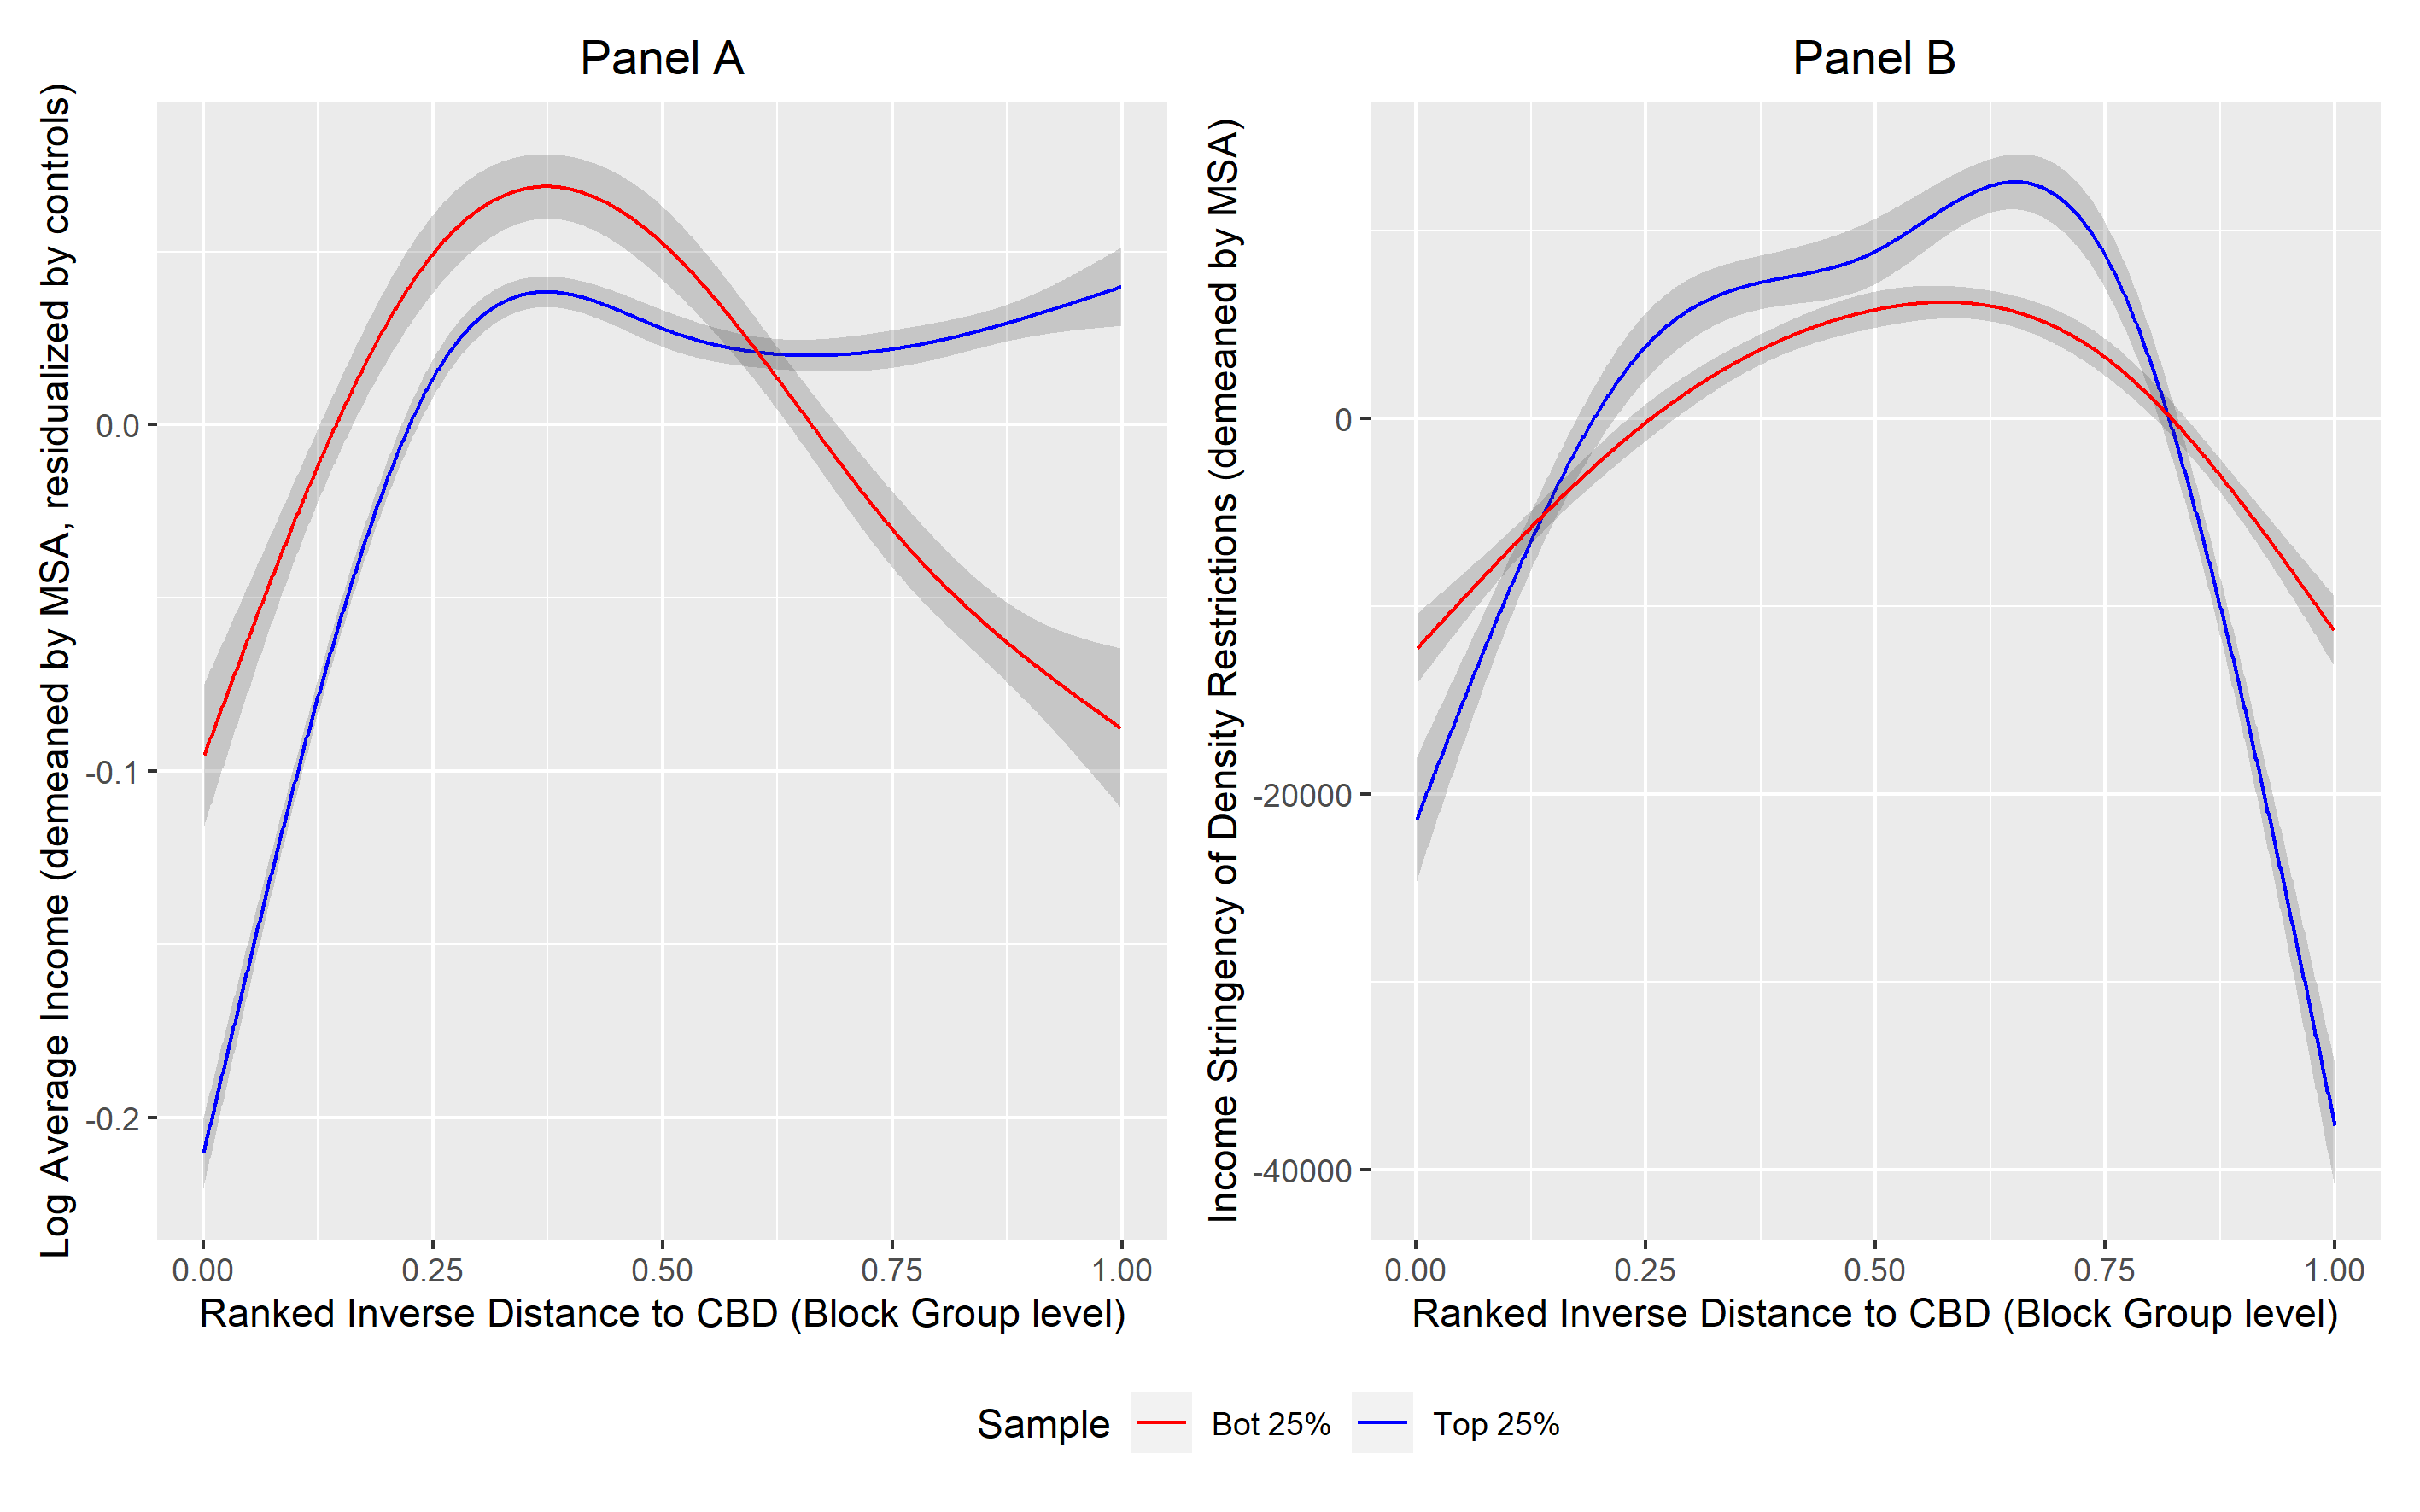
\includegraphics[width=\textwidth]{CBD_combined.png}
			\caption{Plot of cublic spline $\mathbf{S}$ with 5 knots, estimated with the \textit{mgcv} package in R \citep{gampackage}. The specification in Panel A replaces ranked housing unit density with a ranking of (inverse) distance to CBD in Equation \eqref{Specification:IncomeSortingStrong}. Panel B does the same with excluded controls and stringency as the independent variable, demeaned by city and measured in 2012 US dollars. The residualized version of Panel B (mirroring Panel B of Figure \ref{Figure:IncomeSortingStrong}) is omitted as they look qualitatively identical. 95 \% confidence sets are reported.  }\label{Figure:CBD} 
		\end{center}
	\end{figure}
	
	\paragraph*{Across Time}  Strong differences in the income density gradient were even larger in the past. Using the 2008-2012 pooled ACS, the single crossing property in Panel B of Figure \ref{FIncomeDens} holds both conditional on and unconditional on controls. This suggests rapid gentrification happening in the high density neighborhoods of expensive cities. 
		
\end{document}